\subsection{List of Abbreviations}
\label{appendix:list_of_abbrevations}

\renewcommand{\thetable}{A\arabic{table}} % Prefix "A" for Appendix tables
\setcounter{table}{0} % Reset table counter

\begin{table}[H]
    \centering
    \caption[List of Abbreviations]{List of Abbreviations.}
    \label{table:abbreviations}
    \fontsize{8.5}{10.8}\selectfont
    \begin{subtable}[t]{0.49\textwidth}
        \centering
        \begin{tabular}{lp{0.64\textwidth}}
        \toprule
        \textbf{Abbreviation} & \textbf{Definition} \\
        \midrule
        ADAM & Adaptive Moment Estimation \\
        AE & Auto-Encoder \\
        AIS & Average Internal Score \\
        AI & Artificial Intelligence \\
        ANN & Artificial Neural Network \\
        ARIMA & AutoRegressive Integrated Moving Average \\
        AUROC & Area Under the ROC Curve \\
        BGLM & Bayesian Generalized Linear Model \\
        B-HANN & Bootstrapped Hybrid Artificial Neural Network \\
        BIC & Bayesian Information Criterion \\
        BNN & Bayesian Neural Network \\
        B-SLR & Bibliometric Systematic Literature Review \\
        B-SVR & Bayesian Support Vector Regression \\
        BSTS & Bayesian Structural Time-Series \\
        B-TABL & Bayesian Temporal Augmented Bilinear Network \\
        CDF & Cumulative Distribution Functions \\
        cGAN & Conditional Generative Adversarial Networks \\
        CHMM & Continuous Hidden Markov Models \\
        CNN & Convolutional Neural Networks \\
        CoV & Coefficient of Variation \\
        CPS & Conformal Predictive System \\
        CRPS & Continuous Ranked Probability Score \\
        CVaR / ES & Conditional Value at Risk / Expected Shortfall \\
        CWC & Coverage Widthbased Criterion \\
        DCNN & Deep Convolutional Neural Network \\
        DNN & Deep Neural Network \\
        DQ & Dynamic Quantile \\
        ECE & Expected Calibration Error \\
        ECD & Expected Calibration Distance \\
        EGARCH & Exponential GARCH \\
        EMH & Efficient Market Hypothesis \\
        ESVM & Echo State Volatility Model \\
        EWSVM & Enhanced Weighted Support Vector Machine \\
        FINAW & Forecasting Interval Normalized Average Width \\
        FF-ANN & Feed-Forward Artificial Neural Network \\
        FFNN & Feed-Forward Neural Network \\
        GAN & Generative Adversarial Network \\
        GA & Genetic Algorithms \\
        GBHM & Bayesian General Heteroskedasticity Model \\
        GMV & Global Minimum Variance \\
        GP & Gaussian Process \\
        GPMCH & Gaussian Process Mixture Conditional Heteroscedasticity \\
        GPR & Gaussian Processes Regression \\
        GARCH & Generalized Autoregressive Conditional Heteroskedasticity \\
        GRU & Gated Recurrent Units \\
        HMM & Hidden Markov Model \\
        IMF & Intrinsic Mode Functions \\
        ITM & In-The-Money \\
        IVOL & Implied Volatility \\
        \bottomrule
        \end{tabular}
    \end{subtable}
    \hfill
    \begin{subtable}[t]{0.49\textwidth}
        \centering
        \begin{tabular}{lp{0.63\textwidth}}
        \toprule
        \textbf{Abbreviation} & \textbf{Definition} \\
        \midrule
        LOB & Limit Order Books \\
        LOO-CCPS & Leave-One-Out Cross-Conformal Predictive System \\
        LSTM & Long Short-Term Memory \\
        MAE & Mean Absolute Error \\
        MAPE & Mean Absolute Percentage Error \\
        MC & Mean Coverage \\
        MCUB & Multi-Class Undersampling-Based Bagging \\
        MCHMM & Multi-Layer Coupled Hidden Markov Model \\
        MCMC & Markov Chain Monte Carlo \\
        MLP & Multilayer Perceptron \\
        ML & Machine Learning \\
        MNF & Minimum Norm Filter \\
        MSEV & Mean Squared Error of Variance \\
        MWP & Mean Width Percentage \\
        NLL & Negative Log-Likelihood \\
        NSE & Nash–Sutcliffe Model Efficiency Coefficient \\
        OLMAR & Online Moving Average Reversion \\
        OTM & Out-Of-The-Money \\
        PAMR & Passive-Aggressive Mean Reversion \\
        PDF & Probability Density Functions \\
        PGM & Probabilistic Graphical Model \\
        PICP & Prediction Interval Coverage Probability \\
        PINAW & Prediction Interval Normalized Average Width \\
        PIP & Perceptually Important Points \\
        PNN & Probabilistic Neural Network \\
        PredACGAN & Predictive Auxiliary Classifier GAN \\
        PTPP & Probabilistic Trend Prediction Precision \\
        QL & Quantile Loss \\
        QR & Quantile Regression \\
        RDL & Recurrent Dictionary Learning \\
        RELM & Regularized Extreme Learning Machine \\
        RNN & Recurrent Neural Network \\
        RMSCE & Root Mean Squared Calibration Error \\
        RMSE & Root Mean Squared Error \\
        RSMAN & Risk-Sensitive Multi Agent Network \\
        RT & Reparametrization Trick \\
        SAVING & Sentiment-Aware Volatility Forecasting \\
        SGD & Stochastic Gradient Descent \\ 
        SHOA & Spotted Hyena Optimization Algorithm \\
        SLR & Systematic Literature Review \\
        SSA & Singular Spectrum Analysis \\
        SSE & Sum of Squared Errors \\
        SVM & Support Vector Machines \\
        SVR & Support Vector Regression \\
        TARCH & Threshold GARCH \\
        TCN & Temporal Convolutional Network \\
        TVaR & Tail Value at Risk \\
        UCRP & Uniform Constant Rebalanced Portfolio \\
        VaR & Value at Risk \\
        VAE & Variational Autoencoder \\
        VDM & Variational Mode Decomposition \\
        VOGN & Variational Online Gauss-Newton \\
        XAI & Explainable AI \\
        &\\
        \bottomrule
        \end{tabular}
    \end{subtable}
\end{table}

\subsection{Search Queries Used for Literature Search in Scientific Databases}
\label{appendix:search_queries}
\renewcommand{\thetable}{B\arabic{table}} % Prefix "B" for Appendix tables
\setcounter{table}{0} % Reset table counter
\begin{table}[H]
    \centering
    \caption[Database-Specific Search Queries Using Identical Keywords]{Database-Specific Search Queries Using Identical Keywords.}
    \label{table:database_search_queries}
    \fontsize{8.5}{10.8}\selectfont
    \begin{adjustbox}{width=1\textwidth,center}
    \begin{tabular}{lp{0.85\textwidth}}
        \toprule
        \textbf{Database} & \textbf{Search Query} \\
        \midrule
        \text{Web of Science} & \texttt{TS=("AI" OR "ML" OR "Artificial intelligence" OR "Machine learning" OR "deep learning" OR "reinforcement learning" OR "supervised learning") AND TS=("probabilistic" OR "uncertainty quantification" OR "prediction interval*" OR "confidence interval*" OR "distributional forecast" OR "bayesian" OR "Gaussian process" OR "Undirected graphical model*" OR "Markov Network*" OR "Markov random field*" OR "Probabilistic Graphical Model*" OR "Variational inference" OR "Monte Carlo inference" OR "Hidden Markov model*" OR "Gaussian mixture model*" OR "Variational Autoencoder*" OR "Dirichlet Process") AND TS=("Forecast*" OR "predict*" OR "estimat*") AND TS=("cryptocurrency" AND "bitcoin" OR "foreign exchange" OR "equity market*" OR "stock price*" OR "stock market*" OR "stock return*" OR "stock index" OR "stock indices" OR "commodities" OR "value-at-risk" OR "value at risk" OR "CVaR" OR "expected shortfall" OR "forex" OR "financial time series" OR "stock trend*" OR "implied volatility" OR "realized volatility" OR ("volatility" AND "financ*"))} \\
        \addlinespace
        \hdashline[0.2pt/3pt]
        \addlinespace
        \text{Scopus} & \texttt{( TITLE-ABS-KEY ( "AI" OR "ML" OR "Artificial intelligence" OR "Machine learning" OR "deep learning" OR "reinforcement learning" OR "supervised learning" ) AND TITLE-ABS-KEY ( "probabilistic" OR "bayesian" OR "Gaussian process" OR "uncertainty quantification" OR "prediction interval*" OR "confidence interval*" OR "distributional forecast" OR "Undirected graphical model*" OR "Markov Network*" OR "Markov random field*" OR "Probabilistic Graphical Model*" OR "Variational inference" OR "Monte Carlo dropout" OR "Hidden Markov model*" OR "Gaussian mixture model*" OR "Variational Autoencoder*" OR "Dirichlet Process") AND TITLE-ABS-KEY ( "Forecast*" OR "predict*" OR "estimat*") AND TITLE-ABS-KEY ( "cryptocurrency" OR "bitcoin" OR "foreign exchange" OR "equity market*" OR "stock price*" OR "stock return*" OR "stock market*" OR "stock return*" OR "stock index" OR "stock indices" OR "commodities" OR "value-at-risk" OR "value at risk" OR "CVaR" OR "expected shortfall" OR "forex" OR "financial time series" OR "stock trend*" OR "implied volatility" OR "realized volatility" OR ( "volatility" AND "financ*" ))) AND ( LIMIT-TO ( DOCTYPE,"ar" ) OR LIMIT-TO ( DOCTYPE,"re" ) ) AND ( LIMIT-TO ( LANGUAGE,"English" ) )} \\
        \addlinespace
        \hdashline[0.2pt/3pt]
        \addlinespace
        \text{ProQuest} & \texttt{(SUMMARY,IF,TITLE(("AI" OR "ML" OR "Artificial intelligence" OR "Machine learning" OR "deep learning" OR "reinforcement learning" OR "supervised learning") AND ("probabilistic" OR "bayesian" OR "Gaussian process" OR "uncertainty quantification" OR ("prediction interval" OR "prediction intervals") OR ("confidence interval" OR "confidence intervals") OR "distributional forecast" OR "Undirected graphical model*" OR ("markov network") OR "Markov random field*" OR "Probabilistic Graphical Model*" OR "Variational inference" OR "Monte Carlo inference" OR "Hidden Markov model*" OR "Gaussian mixture model*" OR "Variational Autoencoder*" OR "Dirichlet Process") AND ("Forecast*" OR "predict*" OR "estimat*") AND ("cryptocurrency" OR "bitcoin" OR "foreign exchange" OR ("equity market" OR "equity markets") OR ("stock price" OR "stock prices") OR ("stock market" OR "stock markets") OR ("stock returned" OR "stock returns") OR "stock return" OR "stock index" OR "stock indices" OR "commodities" OR "value-at-risk" OR "value at risk" OR "CVaR" OR "expected shortfall" OR "forex" OR "financial time series" OR "stock trend*" OR "implied volatility" OR "realized volatility" OR ("volatility" AND "financ*"))) AND stype.exact("Scholarly Journals" OR "Dissertations \& Theses") AND la.exact("ENG")) AND (pd(19920101-20241016) AND PEER(yes))} \\
        \addlinespace
        \hdashline[0.2pt/3pt]
        \addlinespace
        \text{IEEE Xplore} & \texttt{("AI" OR "ML" OR "Artificial intelligence" OR "Machine learning" OR "deep learning" OR "reinforcement learning" OR "supervised learning") AND ("probabilistic" OR "uncertainty quantification" OR "prediction interval" OR "prediction intervals" OR "confidence interval*" OR "distributional forecast" OR "bayesian" OR "Gaussian process" OR "Undirected graphical model" OR "Undirected graphical models" OR "Markov Network" OR "Markov Networks" OR "Markov random field*" OR "Markov random field" OR "Markov random fields" OR "Probabilistic Graphical Model" OR "Probabilistic Graphical Models" OR "Variational inference" OR "Monte Carlo dropout" OR "Hidden Markov model" OR "Hidden Markov models" OR "Gaussian mixture model" OR "Gaussian mixture models" OR "Variational Autoencoder" OR "Variational Autoencoders" OR "Dirichlet Process") AND ("Forecast*" OR "predict*" OR "estimat*") AND ("cryptocurrency" OR "bitcoin" OR "foreign exchange" OR "equity market*" OR "stock price*" OR "stock market*" OR "stock return" OR "stock returns" OR "stock index" OR "stock indices" OR "commodities" OR "value-at-risk" OR "value at risk" OR "CVaR" OR "expected shortfall" OR "forex" OR "financial time series" OR "stock trend*" OR "implied volatility" OR "realized volatility" OR ( "volatility" AND "financ*" ))} \\
        \bottomrule
    \end{tabular}
    \end{adjustbox}
\end{table}

\subsection{Screening Process in Detail}
\label{appendix:screening_process_with_ai}

\renewcommand{\thefigure}{C\arabic{figure}} % Prefix "C" for Appendix figures
\setcounter{figure}{0} % Reset figure counter
This appendix provides a detailed overview of the screening process employed during each phase in the systematic literature review. All associated code and implementation details are available at: \url{https://github.com/tjespe/literature-review}

\textbf{Screening Phase 1: Initial Screening} \\
Figure \ref{fig:screening_process_phase_1} illustrates the first screening phase, where a Python based workstream in Jupiter Notebook was used to streamline the initial screening. The figure shows two examples of presented papers to the reviewers in Screening Phase 1. Researchers are prompted with a choice to include or exclude the paper based on the title, summary, keywords, and abstract, together with a criteria assessment made by a large language model (“o1-mini” from OpenAI) for assistance.  A link to the PDF of the paper is also included to perform a more thorough scan of the paper in cases of doubt.
\begin{figure}[H]
    \centering
     \begin{subfigure}[b]{0.49\textwidth}
         \centering
         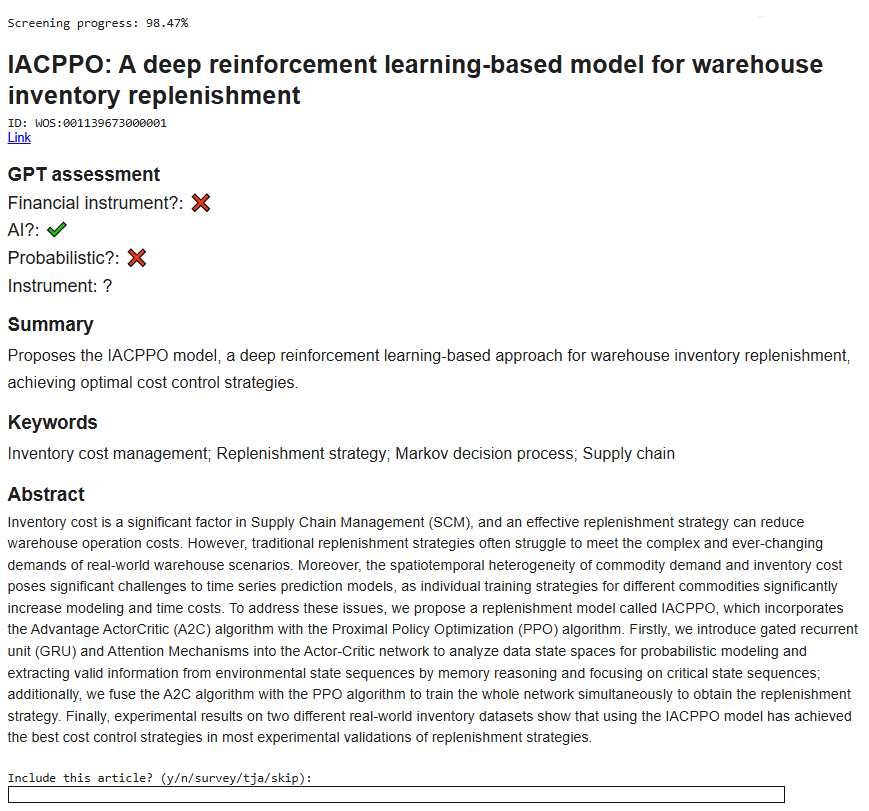
\includegraphics[width=\textwidth]{Images/screening_a.png}
         \caption{Example of paper excluded in Screening Phase 1 due to non compliance with screening criteria.}
         \label{fig:screening_phase_1_rejected}
     \end{subfigure}
     \hfill
     \begin{subfigure}[b]{0.49\textwidth}
         \centering
         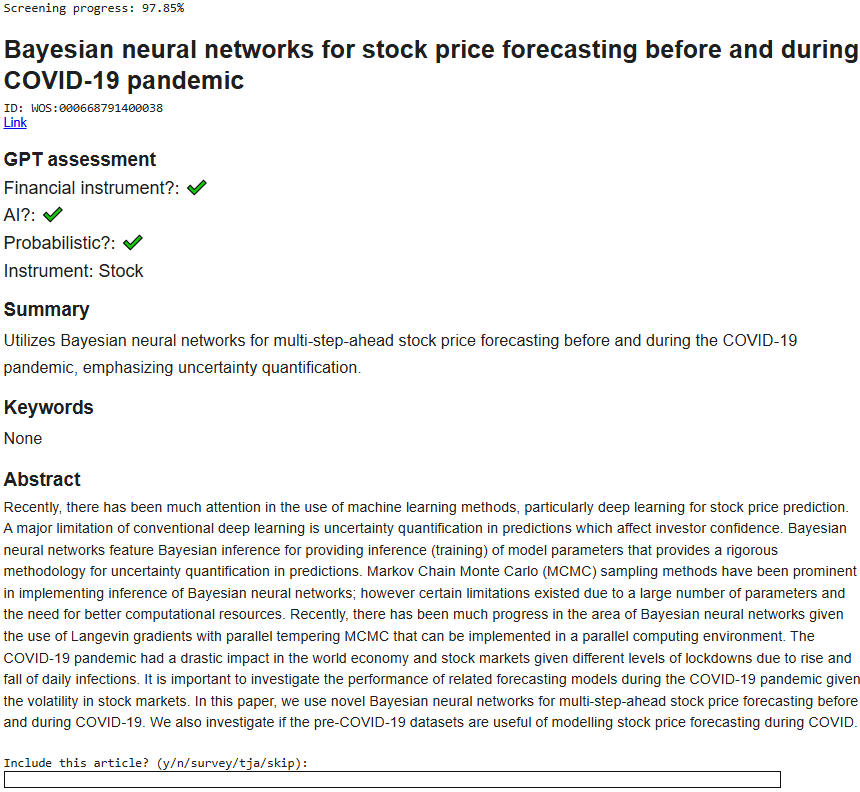
\includegraphics[width=\textwidth]{Images/screening_b2.png}
         \caption{Example of article included after Screening Phase 1 based on relevance and alignment with screening criteria.}
         \label{fig:screening_phase_1_included}
     \end{subfigure}
     \caption[Visualization of streamlined paper screening process methodology during Screening Phase 1]{Examples of presented papers to the reviewer in Screening Phase 1 from Python-based workstream in Jupiter Notebook.}
    \label{fig:screening_process_phase_1}
\end{figure}

\textbf{Screening Phase 2: Full-text screening, Data extraction and Analysis} \\
Figure \ref{fig:screening_process_phase_2} showcases the dynamic table utilized for tagging and systematic data extraction during the full-text screening stage. Key variables were extracted, including model type, target variables, uncertainty estimates assessment and evaluation metrics. Papers not satisfying criteria after all was excluded. This structured data was subsequently loaded into and analyzed using a Python-based  Jupyter Notebook workflow to derive descriptive statistic and perform other analysis. 
\begin{figure}[H]
    \centering
    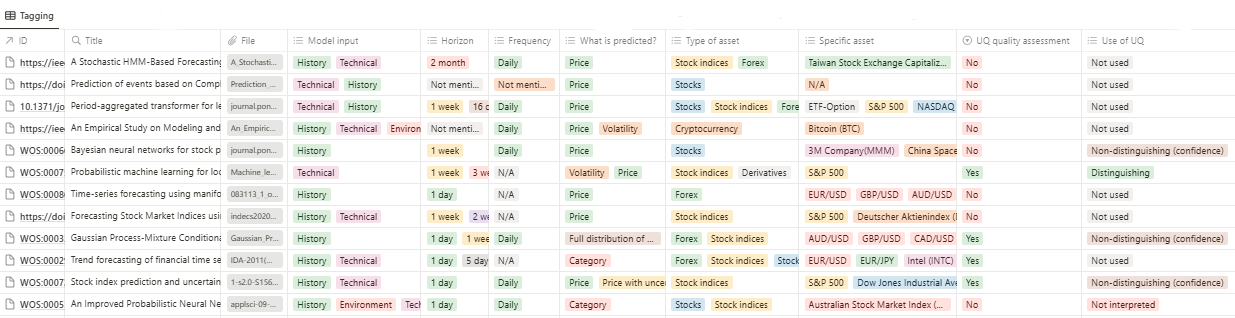
\includegraphics[width=1\linewidth]{Images/screening_process_phase_2.png}
    \caption[Dynamic table for systematic data extraction during full-text screening in Screening Phase 2]{Snapshot of the dynamic table utilized for tagging and systematic data extraction during the full-text screening stage.}
    \label{fig:screening_process_phase_2}
\end{figure}


\subsection{Journals per Category}
\label{appendix:journal_category_mapping}

\renewcommand{\thetable}{D\arabic{table}} % Prefix "D" for Appendix tables
\setcounter{table}{0} % Reset table counter

\begin{table}[H]
    \centering
    \caption[Journal Categories Mapping]{Journals by Category with Corresponding Paper Counts in the Sample.}
    \label{table:journal_categories}
    \small
    \begin{adjustbox}{width=1\textwidth,center}
    \begin{tabular}{p{0.20\textwidth} p{0.80\textwidth}}
        \toprule
        \textbf{Category} & \textbf{Journals} \\  
        \midrule
        Engineering and Technical & IEEE Access (3), Journal of Theoretical and Applied Information Technology (1), CMC-Computers Materials \& Continua (1), Sensors (1), Mobile Information Systems (1) \\
        \addlinespace
        \hdashline[0.2pt/3pt]
        \addlinespace
        Computer Science and Artificial Intelligence & Expert Systems with Applications (4), Neurocomputing (3), Applied Soft Computing (2), International Journal of Data Science and Analytics (1), IEEE Transactions on Systems, Man, and Cybernetics, Part B: Cybernetics (1), Intelligent Data Analysis (1), AI Communications (1), The International Arab Journal of Information Technology (1), IEEE Transactions on Pattern Analysis and Machine Intelligence (1), Cognitive Computation (1), Expert Systems (1), IEEE Transactions on Artificial Intelligence (1), Machine Learning with Applications (1), PeerJ Computer Science (1), Neural Computing and Applications (1), IEEE Transactions on Neural Networks and Learning Systems (1), Engineering Applications of Artificial Intelligence (1), Neural Networks (1), Knowledge-Based Systems (1) \\
        \addlinespace
        \hdashline[0.2pt/3pt]
        \addlinespace
        Multidisciplinary and General Science & PLoS ONE (2), Interdisciplinary Description of Complex Systems (1), Applied Sciences-Basel (1), Trends in Sciences (1), Sustainability (1), Stat (1) \\
        \addlinespace
        \hdashline[0.2pt/3pt]
        \addlinespace
        Economics, Finance, and Business & Quantitative Finance (5), Computational Economics (2), Journal of Financial Reporting and Accounting (1), Digital Finance (1), Journal of Forecasting (1), Journal of Computational Finance (1), Revista Perspectiva Empresarial (1), Research in International Business and Finance (1), Journal of Risk Model Validation (1), SIAM Journal on Financial Mathematics (1) \\
        \addlinespace
        \hdashline[0.2pt/3pt]
        \addlinespace
        Physics and Mathematics & Mathematics (1), Communications in Applied Mathematics and Computational Science (1), Chaos (1), Physica A-Statistical Mechanics and its Applications (1), IAENG International Journal of Applied Mathematics (1), Journal of Statistical Computation and Simulation (1), Technometrics (1), Mathematics and Computers in Simulation (1) \\
        \bottomrule
    \end{tabular}
    \end{adjustbox}
\end{table}




\subsection{Descriptive Table of Key Attributes for Papers in Sample}
\label{appendix:descriptive_table_of_all_articles}

The following table (Table  \ref{appendix:descriptive_table_of_all_articles}1) summarize key attribute of the papers reviewed in this literature review. This includes among other the reference, predicted asset, input data type, prediction horizon, models employed, the use and assessment of uncertainty quantification and whether code is disclosed. This allows for easy comparison of the methods and assessment criteria employed across papers.  

\renewcommand{\thetable}{E\arabic{table}} % Prefix "E" for Appendix tables
\setcounter{table}{0} % Reset table counter
\scriptsize % Adjust font size for the table
\setlength\LTcapwidth{\textheight} % Ensure the caption matches the rotated height

% Rotate the table while allowing it to span multiple pages
\begin{landscape}
    \begin{longtable}{p{0.07\textheight} p{0.07\textheight} p{0.16\textheight} p{0.07\textheight} p{0.07\textheight} p{0.07\textheight} p{0.14\textheight} p{0.09\textheight} p{0.07\textheight} p{0.07\textheight} >{\centering\arraybackslash}p{0.06\textheight} p{0.1\textheight} p{0.03\textheight}}
        \caption[Descriptive Table Summarizing Key Attributes for Papers in Sample]{Descriptive Table Summarizing Key Attributes for Papers in Sample.}
        \label{table:paper_info_summary} \\
        \toprule
        \textbf{Reference} & \textbf{Asset category} & \textbf{Asset} & \textbf{Input} & \textbf{Horizon} & \textbf{Predicted} & \textbf{Prob. AI Model} & \textbf{Composed with ML Model} & \textbf{Composed with Trad. model} & \textbf{Use of UQ} & \textbf{UQ Quality Assessment} & \textbf{Assessment Criteria UQ} & \textbf{Code} \\
        \midrule
        \endfirsthead

        \toprule

        \textbf{Reference} & \textbf{Asset category} & \textbf{Asset} & \textbf{Input} & \textbf{Horizon} & \textbf{Predicted} & \textbf{Prob. AI Model} & \textbf{Composed with ML Model} & \textbf{Composed with Trad. model} & \textbf{Use of UQ} & \textbf{UQ Quality Assessment} & \textbf{Assessment Criteria UQ} & \textbf{Code} \\
        \midrule
        \endhead

        \midrule
        \multicolumn{13}{r}{\textit{Continued on next page}} \\
        \midrule
        \endfoot

        \bottomrule
        \endlastfoot

        \textcite{Almeida2024RiskForecasting} & Crypto-currency & Ethereum portfolio & History, Technical & 1 day & Distribu-tional Forecast, Financial Risk Measure & DeepAR (based on autoregressive RNN) & N/A & N/A & Financial interpretation (e.g. VaR) & Yes & Continuous Ranked Probability Score (CRPS), Elicitability score for VaR & No \\
        \addlinespace
        \hdashline[0.2pt/3pt]
        \addlinespace
        
        \textcite{Chandrasekara2019pnn} & Stock indices, Stocks & Australian Stock Market Index (AORD), S\&P 500, Sri Lankan Stock Market Index (ASPI) & Environment, History, Technical & 1 day & Category & Probabilistic Neural Network (PNN) & multi-class undersampling-based bagging (MCUB) & N/A & Not interpreted & No & N/A & No \\
        \addlinespace
        \hdashline[0.2pt/3pt]
        \addlinespace
        
        \textcite{Daniali2021} & Volatility index & Volatility Index (VIX) & History, Technical & 1 day & Price, Volatility & Deep Convolutional Neural Network (DCNN) & N/A & Conditional Variance model & Not used & No & N/A & No \\
        \addlinespace
        \hdashline[0.2pt/3pt]
        \addlinespace
        
        \textcite{DeSpiegeleer2018gpr} & Derivatives & S\&P 500 American Options, S\&P 500 European Options & Environment, History, Technical & Not mentioned & Distribu-tional Forecast & Gaussian Process Regression (GPR) & N/A & N/A & Not interpreted & No & N/A & No \\
        \addlinespace
        \hdashline[0.2pt/3pt]
        \addlinespace
        
        \textcite{Dixon2022Industrial} & Stocks & International Business Machines (IBM) & History & 1 day, 5 days & Distribu-tional Forecast & Bayesian exponential smoothed RNNs (Bayes ES-RNN) (BNN) & N/A & N/A & Non-distinguishing (confidence) & Yes & Coverage probabillty & No \\
        \addlinespace
        \hdashline[0.2pt/3pt]
        \addlinespace
        
        \textcite{Fatouros2023DeepVaR} & Portfolio & AUD/USD, EUR/USD, GBP/USD, USD/JPY & History, Technical & 1 day & Distribu-tional Forecast, Financial Risk Measure & DeepAR (based on autoregressive RNN) & N/A & N/A & Financial interpretation (e.g. VaR) & Yes & Christoffersen’s Test, Conditional Coverage Test, Dynamic Quantile (DQ), Firm Loss, Quadratic Loss (QL), Smooth Loss, Unconditional Coverage Test & Yes \\
        \addlinespace
        \hdashline[0.2pt/3pt]
        \addlinespace
        
        \textcite{Golnari2024Cryptocurrency} & Crypto-currency & Bitcoin (BTC), Cardano (ADA), Ethereum (ETH), Litecoin (LTC), Polkadot (DOT), Stellar (XLM), Tron (TRX) & History, Technical & 5 minutes & Distribu-tional Forecast & Probabilistic Gated Recurrent Units (P-GRU) & N/A & N/A & Non-distinguishing (confidence) & No & N/A & Yes \\
        \addlinespace
        \addlinespace
        \addlinespace
        \addlinespace
        \addlinespace
        \addlinespace
        \addlinespace
        \addlinespace
        \addlinespace
        \addlinespace
        \addlinespace
        \addlinespace
        \addlinespace
        \addlinespace
        \addlinespace
        \addlinespace
        \addlinespace
        \addlinespace
        \hdashline[0.2pt/3pt]
        \addlinespace
       
        \textcite{Grudniewicz2023Application} & Stock indices & Budapest Stock Exhange Index (BUX), Bulgaria Stock Exchange Index (SOFIX), Deutscher Aktienindex (DAX), OMX Riga Index (OMXR), OMX Tallin Index (OMXT), OMX Vilnius Index (OMXV), Prague Stock Exchange Index (PX), S\&P 500, Warsaw Stock Exchange Index (WIG20) & History, Technical & 20 days & Category & Bayesian Generalized Linear Model (BGLM), Naïve Bayes (NB) & N/A & N/A & Not used & No & N/A & No \\
        \addlinespace
        \hdashline[0.2pt/3pt]
        \addlinespace
        
        \textcite{Hassan2024Bitcoin} & Crypto-currency & Bitcoin (BTC) & History & 1 day & Distribu-tional Forecast & Bayesian LSTM with Monte Carlo Drouput & N/A & N/A & Epistemic (Model) & No & N/A & No \\
        \addlinespace
        \hdashline[0.2pt/3pt]
        \addlinespace
        
        \textcite{Hendawy2023} & Stocks & Egyptian Exchange 100 Stocks & Environment, Fundamental, History, Technical & Quarterly & Distribu-tional Forecast & Gaussian Process Regression (GPR) & N/A & N/A & Not used & No & N/A & No \\
        \addlinespace
        \hdashline[0.2pt/3pt]
        \addlinespace
        
        \textcite{Hocht2024gpr} & Capped volatility swaps & Apple Inc. (AAPL), JPMorgan Chase \& Co (JPM), S\&P 500 & Environment, History, Technical & Flexible & Volatility & Gaussian Process Regression (GPR) & N/A & N/A & Not used & No & N/A & No \\
        \addlinespace
        \hdashline[0.2pt/3pt]
        \addlinespace
        
        \textcite{Horenko2020} & Stock indices & Dow Jones Industrial Average (DJI), EURO STOXX 50 (STOXX), FTSE 100, Hang Seng Index (HSI), Nikkei Stock Average (NI225), S\&P 500, Swiss Market Index (SMI) & History, Technical & 1 day & Distribu-tional Forecast, Financial Risk Measure & TV-Entropy & N/A & N/A & Aleatoric (Volatility), Financial interpretation (e.g. VaR) & Yes & Bayesian Information Criteria (BIC), Coverage probabillty, Kupiec’s test, negative log-likelihood (NLL) & Yes \\
        \addlinespace
        \hdashline[0.2pt/3pt]
        \addlinespace
        
        \textcite{Lahmiri2024pnn} & Stock indices, Stocks & Apple Inc. (AAPL), Cisco Systems (CSCO), General Electric (GE), NYSE Composite & History, Sentiment, Technical & 1 day & Category & Probabilistic Neural Network (PNN) & N/A & N/A & Not interpreted & No & N/A & No \\
        \addlinespace
        \hdashline[0.2pt/3pt]
        \addlinespace
        
        \textcite{Law2017Practical} & Bonds, Commodities, Credit Default Swap (CDS) Spreads, Stock indices & CME Gold Front Month Futures, FTSE 100, IBM-CDS 5YR, ICE BRENT Crude Oil Front Month Futures, S\&P 500, UK Gilt 10YR Bond Yield, US Treasury 10YR Bond Yield, WMT-CDS 5YR & History & 1 day & Distribu-tional Forecast & Bayesian Support Vector Regression (B-SVR) & N/A & N/A & Non-distinguishing (confidence) & Yes & Correlation between uncertainty and prediction error & No \\
        \addlinespace
        \addlinespace
        \addlinespace
        \addlinespace
        \hdashline[0.2pt/3pt]
        \addlinespace
        
        \textcite{Li2024DeepAR} & Stocks & Chinese company stocks & History & Flexible & Distribu-tional Forecast & DeepAR with attention (DeepARA) & N/A & N/A & Non-distinguishing (confidence) & Yes & Entropy of probability distribution & No \\
        \addlinespace
        \hdashline[0.2pt/3pt]
        \addlinespace
        
        \textcite{Li2024gpr} & Portfolio & MSCI World Index (MSCI), New York Stock Exchange (NYSE) stock portfolio, S\&P 500, Toronto Stock Exchange (TSE) stock portfolio & History, Technical & 1 day & Distribu-tional Forecast & Graph-Aware Gaussian Process (G4P) & N/A & N/A & Non-distinguishing (confidence) & Yes & Portfolio construction and evaluation & Yes \\
        \addlinespace
        \hdashline[0.2pt/3pt]
        \addlinespace
        
        \textcite{Malagrino2018Forecasting} & Stock indices & Bombay Stock Exchange (BSE 30 SENSEX), Cotation Assistée en Continu (CAC 40), Deutscher Aktienindex (DAX), Dow Jones Industrial Average (DJI), FTSE 100, Hang Seng Index (HSI), Merval (MERV), NASDAQ Composite, NYSE Composite, Nikkei Stock Average (NI225), Shanghai Composite (SSE), Stockholm General (OMXS 30) & Environment, History, Technical & 1 day, 2 days, 20 days & Category & Bayesian Neural Network (BNN) & N/A & N/A & Not interpreted & No & N/A & No \\
        \addlinespace
        \hdashline[0.2pt/3pt]
        \addlinespace
        
        \textcite{Min2023BlackLitterman} & Portfolio, Stocks & S\&P 500 stock portfolio & History & 50 months & Distribu-tional Forecast & Gaussian Process Regression (GPR) & N/A & Black-Litterman & Non-distinguishing (confidence) & Yes & Portfolio construction and evaluation & No \\
        \addlinespace
        \hdashline[0.2pt/3pt]
        \addlinespace
        
        \textcite{Papaioannou2022gpr} & Forex & AUD/USD, CAD/USD, CHF/USD, DKK/USD, EUR/USD, GBP/USD, JPY/USD, NOK/USD, NZD/USD, SEK/USD & History & 1 day & Price & Gaussian Process Regression (GPR) & N/A & N/A & Not used & No & N/A & No \\
        \addlinespace
        \hdashline[0.2pt/3pt]
        \addlinespace
        
        \textcite{Park2014gpr} & Options & KOSPI 200 Index options & Technical & Flexible & Price & Gaussian Process Regression (GPR) & N/A & N/A & Not used & No & N/A & No \\
        \addlinespace
        \addlinespace
        \addlinespace
        \addlinespace
        \addlinespace
        \addlinespace
        \addlinespace
        \hdashline[0.2pt/3pt]
        \addlinespace
        
        \textcite{Park2024UncertaintyAware} & Portfolio, Stocks & KOSPI stocks, NASDAQ stocks, NYSE stocks & History, Technical & Short (milliseconds) & Distribu-tional Forecast & Risk-sensitive multiagent network (RSMAN) & N/A & N/A & Distinguishing & Yes & Portfolio construction and evaluation & No \\
        \addlinespace
        \hdashline[0.2pt/3pt]
        \addlinespace
        
        \textcite{Parker2021BayesianHeteroskedastic} & Stock indices & Dow Jones Industrial Average (DJI) & Environment, History, Technical & Not mentioned & Volatility & Echo State Volatility Model (ESVM) & N/A & N/A & Distinguishing & Yes & Coverage probabillty, MSEV & No \\
        \addlinespace
        \hdashline[0.2pt/3pt]
        \addlinespace
        
        \textcite{Platanios2014gpr} & Forex, Stock indices & AUD/USD, CAD/USD, CHF/USD, Canadian TSX Composite (TSX), Cotation Assistée en Continu (CAC 40), DEM/USD, DKK/USD, Deutscher Aktienindex (DAX), FRF/USD, FTSE 100, GBP/USD, JPY/USD, Nikkei Stock Average (NI225), S\&P 500 & History & 1 day, 1 week, 30 days & Distribu-tional Forecast, Volatility & Non-parametric Bayesian mixture of Gaussian process regression models (GPMCH) & N/A & N/A & Non-distinguishing (confidence) & Yes & RMSE (against squared returns) & No \\
        \addlinespace
        \hdashline[0.2pt/3pt]
        \addlinespace
        
        \textcite{Raúl_PlazaCasado_PradoRomán_2021} & Stock indices & IBerian Index (IBEX) & History, Sentiment & 1 day & Category & Bayesian Network (BN) & N/A & N/A & Non-distinguishing (confidence) & Yes & Success rate & No \\
        \addlinespace
        \hdashline[0.2pt/3pt]
        \addlinespace
        
        \textcite{Risk2018gpr} & Portfolio & N/A & Environment, History & 1 year & Distribu-tional Forecast, Financial Risk Measure & Gaussian Process Regression (GPR) & N/A & N/A & Distinguishing, Financial interpretation (e.g. VaR) & Yes & RMSE (against Harrell-Davis as ground truth) & No \\
        \addlinespace
        \hdashline[0.2pt/3pt]
        \addlinespace
        
        \textcite{Sharma2021} & Stocks & Chinese company stocks, India stocks, UK stocks, USA stocks & History & 1 day & Category, Distribu-tional Forecast & Recurrent Dictionary Learing (RDL) & N/A & N/A & Non-distinguishing (confidence) & Yes & Log-loss & No \\
        \addlinespace
        \hdashline[0.2pt/3pt]
        \addlinespace
        
        \textcite{Suphawan2022gpr} & Stock indices & Stock Exchange Thailand Index (SET) & History, Technical & 1 day & Distribu-tional Forecast & Gaussian Process Regression (GPR) & N/A & N/A & Non-distinguishing (confidence) & No & N/A & No \\
        \addlinespace
        \hdashline[0.2pt/3pt]
        \addlinespace
        
        \textcite{Thawornwong2004pnn} & Portfolio & S\&P 500 stock portfolio & Environment, Fundamental, History, Technical & 1 month & Category & Probabilistic Neural Network (PNN) & N/A & N/A & Not used & No & N/A & No \\
        \addlinespace
        \hdashline[0.2pt/3pt]
        \addlinespace
        
        \textcite{Tian2023} & Volatility index & 10-Year U.S. treasury note volatility index (TYVIX), Crude Oil ETF Volatility Index (COEVI), Volatility Index (VIX) & Environment, History, Technical & Not mentioned & Distribu-tional Forecast, Volatility & Fitting error analysis & Clockwork Recurrent Neural Network (CWRNN), Cuckoo-Search-enhanced Multi-Objective Grey Wolf Optimizer (MOGWOCS) & N/A & Non-distinguishing (confidence) & Yes & PICP (Prediction interval coverage probability), Prediction Interval Normalized Average Width (PINAW), Winkler Score, coverage widthbased criterion (CWC) & No \\
        \addlinespace
        \hdashline[0.2pt/3pt]
        \addlinespace
        
        \textcite{Wang2021gprensemble} & Stock indices & Hang Seng Index (HSI), Nikkei Stock Average (NI225) & History & 1 day & Distribu-tional Forecast & Gaussian Process Regression (GPR) & Enhanced Weighted Support Vector Machine (EWSVM), Recurrent Neural Network (RNN) & Singular Spectrum Analysis (SSA) & Non-distinguishing (confidence) & Yes & Coverage probabillty, MWP (Mean width percentage), Mean width divided by coverage probability & No \\
        \addlinespace
        \hdashline[0.2pt/3pt]
        \addlinespace
        
        \textcite{Wang2021gpr} & Stock indices & Dow Jones Industrial Average (DJI), NASDAQ Composite, S\&P 500 & History, Technical & 1 day & Distribu-tional Forecast & Gaussian Process Regression (GPR) & Auto-Encoder (AE), Long Short Term Memory Neural Network (LSTM), Recurrent Neural Network (RNN), Variational Mode Decomposition (VMD) & N/A & Non-distinguishing (confidence) & Yes & MC (Mean coverage), MWP (Mean width percentage), PICP (Prediction interval coverage probability) & No \\
        \addlinespace
        \hdashline[0.2pt/3pt]
        \addlinespace
        
        \textcite{Wang2024GoldForecasting} & Commodities & Gold price & Environment, History, Sentiment & Not mentioned & Confidence Interval & Quantile Regression Bi-Directional Long Short-Term Memory (QRBiLSTM) & N/A & N/A & Aleatoric (Volatility) & Yes & PICP (Prediction interval coverage probability), Prediction Interval Normalized Average Width (PINAW), Quantile loss (QL), Semi-interval metric, average interval score (AIS) & No \\
        \addlinespace
        \hdashline[0.2pt/3pt]
        \addlinespace
        
        \textcite{Zhang2016} & Stocks & NASDAQ stocks, Second-board Market of Shenzhen Stock Exchange (SZSE) stocks & History, Technical & Flexible & Category & Probabilistic Support Vector Machine (PSVM) & AdaBoost, Genetic Algorithm (GA) & N/A & Not interpreted & No & N/A & No \\
        \addlinespace
        \hdashline[0.2pt/3pt]
        \addlinespace
        
        \textcite{Zmuk2020gpr} & Stock indices & Deutscher Aktienindex (DAX), Dow Jones Industrial Average (DJI), NASDAQ Composite, Nikkei Stock Average (NI225), S\&P 500 & History, Technical & 1 month, 1 week, 2 weeks & Price & Gaussian Process Regression (GPR) & N/A & N/A & Not used & No & N/A & No \\
        \addlinespace
        \addlinespace
        \addlinespace
        \addlinespace
        \addlinespace
        \addlinespace
        \addlinespace
        \addlinespace
        \hdashline[0.2pt/3pt]
        \addlinespace
        
        \textcite{arian2022encoded} & Portfolio, Stocks & Frankfurt Stock Exchange (FSE) stock portfolio, London Stock Exchange (LSE) stock portfolio, S\&P 500 & History, Technical & 1 day & Distribu-tional Forecast, Financial Risk Measure & Variational Auto-encoder (VAE) & N/A & N/A & Aleatoric (Volatility), Financial interpretation (e.g. VaR) & Yes & Christoffersen’s Test, Conditional Coverage Test, Independence Test, Kupiec’s test, Lopez' loss function, Unconditional Coverage Test & Yes \\
        \addlinespace
        \hdashline[0.2pt/3pt]
        \addlinespace
        
        \textcite{cao2019multi} & Forex, Stock indices & S\&P 500 & History, Technical & 1 week & Category & Multi-Layer Coupled Hidden Markov Model (MCHMM) & N/A & N/A & Not interpreted & No & N/A & No \\
        \addlinespace
        \hdashline[0.2pt/3pt]
        \addlinespace
        
        \textcite{caprioli2023quantifying} & Portfolio & Total Market Index Emerging Markets, Total Market Index Europe, Total Market Index Italy, Total Market Index US & History, Technical & 1 year & Financial Risk Measure & Variational Auto-encoder (VAE) & N/A & multi-factor Vasicek model & Financial interpretation (e.g. VaR) & Yes & Te largest eigenvalue of the correlation matrix & No \\
        \addlinespace
        \hdashline[0.2pt/3pt]
        \addlinespace
        
        \textcite{chandra2021bayesian} & Stocks & 3M Company(MMM), China Spacesat Company Limited (600118.SS), Commonwealth Bank of Australia (CBA.AX), Daimler AG (DAI. DE) & History & 1 week & Distribu-tional Forecast & Langevin-gradient Bayesian neural networks (BNN) with parallel tempering Markov Chain Monte Carlo (MCMC) & N/A & N/A & Non-distinguishing (confidence) & No & Confidence interval & Yes \\
        \addlinespace
        \hdashline[0.2pt/3pt]
        \addlinespace
        
        \textcite{choudhury2020enhancing} & Stocks & Adobe (ADBE), Amazon (AMZN), Apple Inc. (AAPL), Cerner Corporation (CERN), Costco (COST), Facebook (FB), Fastenal Company (FAST), Google (GOOG), Hasbro Inc (HAS), IDEXX Laboratories Inc. (IDXX), Intel (INTC) & History, Technical & 7 minutes & Price & Variational Auto-encoder (VAE) & Long Short Term Memory Neural Network (LSTM) & N/A & Not used & No & N/A & No \\
        \addlinespace
        \hdashline[0.2pt/3pt]
        \addlinespace
        
        \textcite{cocco2021predictions} & Crypto-currency & Bitcoin (BTC), Ethereum (ETH) & Technical & 1 day, 1 month, 2 weeks & Distribu-tional Forecast & BNN-SVR, Bayesian Neural Network (BNN) & N/A & N/A & Non-distinguishing (confidence) & No & N/A & No \\
        \addlinespace
        \addlinespace
        \addlinespace
        \addlinespace
        \addlinespace
        \addlinespace
        \addlinespace
        \addlinespace
        \addlinespace
        \addlinespace
        \addlinespace
        \addlinespace
        \addlinespace
        \addlinespace
        \addlinespace
        \addlinespace
        \hdashline[0.2pt/3pt]
        \addlinespace
        
        \textcite{eriolu2020bootstrapped} & Stock indices & S\&P 500 & History & 1 day & Distribu-tional Forecast & Bootstrapped Hybrid Artificial Neural Network (B-HANN) & N/A & N/A & Non-distinguishing (confidence) & Yes & Reliability Evaluation (RE), lower bound closeness (LBC), mean of closeness (MC), sharpness evaluation (SE), upper bound closeness (LBC) & No \\
        \addlinespace
        \hdashline[0.2pt/3pt]
        \addlinespace
        
        \textcite{govindasamy2014prediction} & Stocks & N/A & History, Technical & Not mentioned & Price & PECEP (Combo of Complex Event Processing [CEP] and Probabilistic Fuzzy Logic [PFL]) & N/A & N/A & Not used & No & N/A & No \\
        \addlinespace
        \hdashline[0.2pt/3pt]
        \addlinespace
        
        \textcite{hortua2024forecasting} & Derivative index & Volatility Index (VIX) & History & Not mentioned & Distribu-tional Forecast & Bayesian Neural Network (BNN), WaveNet & Temporal Convolutional Network (TCN), Transformers & N/A & Distinguishing & Yes & Calibration diagrams, PICP (Prediction interval coverage probability), RMSCE, Scaling factor & No \\
        \addlinespace
        \hdashline[0.2pt/3pt]
        \addlinespace
        
        \textcite{jang2018empirical} & Crypto-currency & Bitcoin (BTC) & Environment, History, Technical & Not mentioned & Price, Volatility & Bayesian neural networks (BNNs) & N/A & N/A & Not used & No & N/A & No \\
        \addlinespace
        \hdashline[0.2pt/3pt]
        \addlinespace
        
        \textcite{jang2018generative} & Options & S\&P 100 American put options & Technical & 1 day, 1 week & Price & Generative Bayesian Neural Network (Gen-BNN) & N/A & N/A & Not used & No & N/A & No \\
        \addlinespace
        \hdashline[0.2pt/3pt]
        \addlinespace
        
        \textcite{kim2023portfolio} & Portfolio & NASDAQ 100 stocks portfolio, S\&P 500 stock portfolio & History, Technical & 1 month & Category & Predictive Auxiliary Classifier Generative Adversarial Networks (PredACGAN) & N/A & N/A & Non-distinguishing (confidence) & Yes & Entropy of probability distribution & Yes \\
        \addlinespace
        \hdashline[0.2pt/3pt]
        \addlinespace
        
        \textcite{lee2021estimation} & Stock indices & NASDAQ-100 Future Index & History, Technical & 1 week & Distribu-tional Forecast & Conditional Generative Adversarial Network (CGAN) & N/A & N/A & Non-distinguishing (confidence) & Yes & Correlation between uncertainty and prediction error, Portfolio construction and evaluation & Yes \\
        \addlinespace
        \hdashline[0.2pt/3pt]
        \addlinespace
        
        \textcite{li2010stochastic} & Forex, Stock indices & Taiwan Stock Exchange Capitalization Weighted Stock Index (TAIEX) & History, Technical & 2 month & Price & Stochastic Hidden Markov Model (HMM) & N/A & N/A & Not used & No & N/A & No \\
        \addlinespace
        \addlinespace
        \addlinespace
        \addlinespace
        \addlinespace
        \hdashline[0.2pt/3pt]
        \addlinespace
        
        \textcite{li2020multivariate} & Commodities & Soybean Futures & Environment, Fundamental, History, Technical & Not mentioned & Price & Multimodal Variational Autoencoder (VAE) & Long Short Term Memory Neural Network (LSTM), Recurrent Neural Network (RNN) & N/A & Not used & No & N/A & No \\
        \addlinespace
        \hdashline[0.2pt/3pt]
        \addlinespace
        
        \textcite{magris2023bayesian} & Stocks & Nasdaq Nordic Helsinki Exchange Stocks & History, Technical & Short (milliseconds) & Category & Bayesian temporal attention augmented bilinear network (B-TABL) & N/A & N/A & Non-distinguishing (confidence) & Yes & Expected Calibration Distance (ECD), Expected Calibration Error (ECE) & No \\
        \addlinespace
        \hdashline[0.2pt/3pt]
        \addlinespace
        
        \textcite{park2011trend} & Forex, Stock indices, Stocks & Boeing (BA), EUR/JPY, EUR/USD, FTSE 100, Intel (INTC), S\&P 500, US-Treasury Bill 5YR, Walmart (WMT) & History, Technical & 1 day, 5 days & Category & Continuous Hidden Markov Model (CHMM) & N/A & PIPs Detection Algorithm & Not used & Yes & Probabilistic Trend Prediction Precision (PTPP) & No \\
        \addlinespace
        \hdashline[0.2pt/3pt]
        \addlinespace
        
        \textcite{qin2016collective} & Stocks & American Stocks (e.g. AT\&T Inc (T), Apple Inc. (AAPL), Boeing (BA)), Chinese Stocks (e.g CN Eastern Airlines (600115SS), CN Medicine \& Health (600056SS)) & Technical & 1 day & Category & Probabilistic Graphical Model (PGM) & N/A & N/A & Not used & No & N/A & No \\
        \addlinespace
        \hdashline[0.2pt/3pt]
        \addlinespace
        
        \textcite{salama2024gan} & Stocks & Axis Bank (AXISBANK), Bharat Heavy Electricals (BHEL), Container Store Group (TSC), Maruti (MARUTI), Tata Steel (TATASTEEL), Wipro (WIPRO) & History, Technical & Short (milliseconds) & Price & Conditional Generative Adversarial Network (CGAN) & Spotted Hyena Optimization Algorithm (SHOA) & N/A & Not used & No & N/A & No \\
        \addlinespace
        \hdashline[0.2pt/3pt]
        \addlinespace
        
        \textcite{sher2023exploiting} & Stocks & Apple Inc. (AAPL), Broadcom Inc. (AVGO), Microsoft Corporation (MSFT), Nvidia Corporation (NVDA), Taiwan Semiconductor Manufacturing Company Limited (LSM) & History & Not mentioned & Category & Hidden Markov Model (HMM) & N/A & N/A & Not used & No & N/A & Yes \\
        \addlinespace
        \addlinespace
        \addlinespace
        \addlinespace
        \addlinespace
        \addlinespace
        \addlinespace
        \addlinespace
        \addlinespace
        \hdashline[0.2pt/3pt]
        \addlinespace
        
        \textcite{soleymani2022longterm} & Stocks & Advanced Micro Devices (AMD), Amazon (AMZN), Apple Inc. (AAPL), Google (GOOG), Microsoft Corporation (MSFT), Nvidia Corporation (NVDA), Pfizer (PFE), Shopify (SHOP), Walmart (WMT) & History, Technical & 10 days, 15 days, 20 days, 30 days, 5 days & Distribu-tional Forecast & Deep Bayesian neural networks (BNNs) & temporal generative adversarial neural networks (t-GAN) & N/A & Fed into other model & No & N/A & No \\
        \addlinespace
        \hdashline[0.2pt/3pt]
        \addlinespace
        
        \textcite{su2022hmm} & Stock indices & Hang Seng Index (HSI) & History, Technical & 1 month, 3 month, 6 month & Category, Price & Hidden Markov Model (HMM) & k-means clustering & N/A & Not used & No & N/A & No \\
        \addlinespace
        \hdashline[0.2pt/3pt]
        \addlinespace
        
        \textcite{tang2024period} & Forex, Options, Stock indices, Stocks & Chinese Securities Index (CSI 300), ETF-Option, Exchange rates, NASDAQ Composite, S\&P 500 & History, Technical & 1 week, 16 days, 32 days, 64 days & Price & Variational Auto-encoder (VAE) & Attention & N/A & Not used & No & N/A & Yes \\
        \addlinespace
        \hdashline[0.2pt/3pt]
        \addlinespace
        
        \textcite{tegner2021probabilistic} & Derivatives, Stock indices & S\&P 500 & Technical & 1 week, 3 weeks & Distribu-tional Forecast, Volatility & Bayesian GPR & N/A & N/A & Distinguishing & Yes & N/A & Yes \\
        \addlinespace
        \hdashline[0.2pt/3pt]
        \addlinespace
        
        \textcite{vuletic2024finGAN} & Stock indices, Stocks & American stocks (e.g. Amazon (AMZN), Nike (NKE), Pfizer (PFE)), ETFs (e.g. XKL (IBM TER), XLB (ECL IP), XLY (AMZN HD NKE)) & Environment, History, Technical & Not mentioned & Distribu-tional Forecast & Conditional Generative Adversarial Network (CGAN) & N/A & N/A & Non-distinguishing (confidence) & Yes & Portfolio construction and evaluation & No \\
        \addlinespace
        \hdashline[0.2pt/3pt]
        \addlinespace
        
        \textcite{wang2020fastconformal} & Stocks & N/A & History, Technical & Not mentioned & Distribu-tional Forecast & Leave-One-Out Cross-Conformal Predictive System (LOO-CCPS) & N/A & N/A & Non-distinguishing (confidence) & Yes & Coverage probabillty, e continuous ranked probability score (CRPS) & No \\
        \addlinespace
        \hdashline[0.2pt/3pt]
        \addlinespace
        
        \textcite{xing2019sentiment} & Stocks & Aegon Ltd (AGN), Alibaba-group (BABA), Amazon (AMZN), Apple Inc. (AAPL), Goldman Sachs Group (GS), Google (GOOG), Pfizer (PFE), Stamper Oil \& Gas Corp (STMP), Starbucks (SBUX), Tesla (TSLA) & History, Sentiment, Technical & 1 day & Volatility & Variational Auto-encoder (VAE) & Recurrent Neural Network (RNN) & N/A & Aleatoric (Volatility) & Yes & negative log-likelihood (NLL) & No \\
        \addlinespace
        \hdashline[0.2pt/3pt]
        \addlinespace
        
        \textcite{zhang2019high} & Stock indices & Chinese Securities Index (CSI 300), S\&P 500 & History, Technical & 1 day & Category & Hidden Markov Model (HMM) & N/A & N/A & Not interpreted & No & N/A & No \\
        \addlinespace
        \addlinespace
        \hdashline[0.2pt/3pt]
    \end{longtable}
\end{landscape}


